\section{Experiments}
\label{sec:experiments}
We first examine low-health and cross-task stress tests; Section~\ref{sec:cv17} then studies larger CV17 data with independent calibration. Protocols are reported separately.

\subsection{Protocol, Metrics, and Comparators}
\label{sec:exp_setup}
\paragraph*{Data and models}
The small Common Voice archive~\cite{ardila2020commonvoice} contains 6,714/1,061/459 train/dev/test clips labeled US, England, or Indian accent.\footnote{\url{https://zenodo.org/records/12588635}; archive metadata specify the Mozilla Public Dataset License 1.0.} Official splits are client/clip-disjoint. Seeds 0--4 reserve $1/4$ of training clients as auxiliary. SSL-BS uses frozen wav2vec2-base features and linear heads, with auxiliary BS counts; Mel-CE uses mel-CNNs. Teachers train eight epochs, batch 128, $C=8$; students train 15, with $\alpha=0.7$, $T=2$. Noise $\sigma=1,1.5,2$ gives seed-wise PRV $\varepsilon=2.7102$--$3.1598$, $1.3270$--$1.5432$, $0.8918$--$1.0328$ at $\delta=10^{-5}$.

VCTK~\cite{veaux2017vctk} uses 720 utterances in four accent classes: 360 private, 120 auxiliary, and 120 each for dev/test. All splits are speaker-disjoint; seeds 0--2 each lack a different auxiliary class. BS mel-CNN teachers train four epochs, students five. Poisson $q=1/6$, 24 updates, $C=8$, $\sigma=1$ give PRV $\varepsilon=6.0829038771$, $\delta=10^{-5}$ (Supplement II-A). Runs use PyTorch 2.11, Opacus 1.6 and RTX 5090 GPUs. The full implementation is public.\footnote{\url{https://github.com/code-experimenter-alt/THG_RoD}}

\paragraph*{Common Voice implementation}
The encoder is \texttt{facebook/wav2vec2-base}, revision \texttt{0b5b8e8}: mono 16-kHz audio, at most 12 seconds, final-layer mean-pooled 768 features. Mel inputs have 40 bins/100 frames, per-frequency normalization and stabilizer $10^{-5}$. AdamW uses learning rate $10^{-3}$, weight decay $10^{-4}$. Maximum dev Macro-F1 selects checkpoints, with earliest ties. Initialization/order seeds are $s+1000003$/$s+1000004$.

\begin{table}[t]
\centering\scriptsize\setlength{\tabcolsep}{3pt}
\caption{Common Voice training settings.}
\label{tab:app_default_hyperparams}
\begin{tabular}{lll}\toprule
Setting & Small archive & CV17\\\midrule
Teacher/student epochs & 8 / 15 & 80 / 80\\
Batch size & 128 & 256\\
AdamW learning rate & $10^{-3}$ & 0.03\\
Weight decay & $10^{-4}$ & $10^{-4}$\\
Clip norm $C$ & 8 & 2\\
Noise $\sigma$ & 1, 1.5, 2 & .5, 1, 2, 4, 8\\
PRV $\delta$ & $10^{-5}$ & $10^{-5}$\\
KD $(\alpha,T)$ & $(0.7,2)$ & $(0.7,2)$\\
SSL sampling / duration & 16 kHz / 12 s & 16 kHz / 12 s\\
SSL feature / classifier & 768 / linear & 768 / linear\\
Mel input (alternative) & $40\times100$ & --\\\bottomrule
\end{tabular}
\end{table}

\paragraph*{Paired evaluation}
We report balanced accuracy (BalAcc), Macro-F1, and diagnostic MajPred. Paired KD gain is
\begin{equation}
\Delta_{\mathrm{KD}}=\mathrm{BalAcc}(s_{\mathrm{KD}})-\mathrm{BalAcc}(s_{\mathrm{Hard}}).
\label{eq:kd_gain}
\end{equation}
Tables~\ref{tab:cv_release_routing}, \ref{tab:cross_dataset_summary}, \ref{tab:cv17_teachers}, and~\ref{tab:cv17_students} use percent scores as mean (SD); CV17 health and $\varepsilon$ remain unscaled. SSL/Mel abbreviate SSL-BS/Mel-CE. Branches share the teacher/cache, student initialization, and auxiliary order. Routes reuse selected checkpoints. Mean $\pm$ sample SD describes seed variation; branch equality is not independent evidence of improvement.

\paragraph*{Two kinds of simple route}
T-BAcc selects Hard below teacher-dev BalAcc 0.45, otherwise KD. S-BAcc/S-MF1/S-MajPred select among trained Hard/KD/HAKD students by dev BalAcc/Macro-F1/minimum MajPred, breaking ties in that order. TCRD chooses the objective before student training. No route uses test utility.

\subsection{Small Common Voice: Diagnosis and Transfer}
\label{sec:cv_main_results}

\begin{table}[t]
\centering
\caption{Small Common Voice teachers ($\sigma=1$; five seeds).}
\label{tab:cv_accent_baseline_dp_loss}
\scriptsize\setlength{\tabcolsep}{3pt}
\begin{tabular}{lccc}
\toprule
Teacher / loss & Acc & BalAcc & MF1\\
\midrule
Non-DP Mel / CE & $.547\pm.032$ & $.341\pm.025$ & $.297\pm.050$\\
Non-DP SSL / CE & $.522\pm.020$ & $.355\pm.020$ & $.323\pm.042$\\
DP SSL / CE & $.516\pm.032$ & $.329\pm.011$ & $.275\pm.013$\\
DP SSL / BS & $.408\pm.192$ & $.347\pm.024$ & $.236\pm.118$\\
\bottomrule
\end{tabular}
\end{table}

\begin{table}[t]
\centering
\caption{Small Common Voice: health and student BalAcc (\%).}
\label{tab:cv_release_routing}
\scriptsize\setlength{\tabcolsep}{2pt}
\begin{tabular}{lcccccc}
\toprule
Teacher & $\sigma$ & Health & Hard & KD & HAKD & CTKD\\
\midrule
SSL & 1.0 & 22.3(7.2) & 34.8(4.1) & 34.3(2.0) & 35.4(3.0) & 34.3(2.8)\\
SSL & 1.5 & 21.7(6.6) & 34.8(4.1) & 34.1(1.2) & 35.4(3.2) & 33.8(1.1)\\
SSL & 2.0 & 22.8(5.3) & 34.8(4.1) & 33.7(2.1) & 35.4(3.9) & 33.3(1.7)\\
\midrule
Mel & 1.0 & 21.2(2.3) & 35.2(3.1) & 32.7(0.8) & 33.4(0.6) & 33.0(0.4)\\
Mel & 1.5 & 20.7(1.8) & 35.2(3.1) & 33.1(0.2) & 32.8(0.4) & 33.3(0.1)\\
Mel & 2.0 & 20.2(1.0) & 35.2(3.1) & 33.2(0.1) & 33.0(0.4) & 32.9(0.9)\\
\bottomrule
\end{tabular}
\end{table}

In Table~\ref{tab:cv_accent_baseline_dp_loss}, BS raises DP teacher BalAcc from 0.329 to 0.347 but lowers Macro-F1 from 0.275 to 0.236 and increases seed variation. Neither BS nor the non-DP controls produces uniformly strong teachers.

Table~\ref{tab:cv_release_routing} gives negative mean KD gain for both families. At $\sigma=1,1.5,2$, SSL gains are $-0.0053\pm0.0291$, $-0.0075\pm0.0388$, $-0.0110\pm0.0277$ (two positive seeds each); Mel gains are $-0.0250\pm0.0314$, $-0.0207\pm0.0305$, $-0.0200\pm0.0304$ (one positive each). Repeated seeds across noise levels are not independent partitions. These near-chance results are low-utility stress tests.

\begin{figure}[t]
\centering
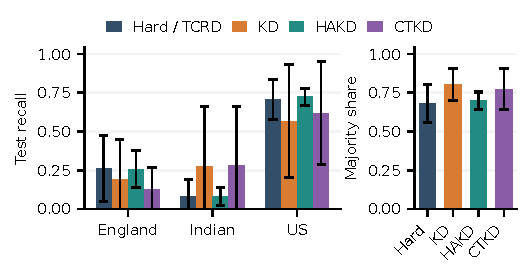
\includegraphics[width=\linewidth]{figure/kd_vs_nokd_seed_only_legend_hatch_two_panels.pdf}
\caption{Small Common Voice SSL-BS: class recall and prediction concentration at $\sigma=1$.}
\label{fig:cv_perclass_kd_diagnostic}
\end{figure}
\begin{figure}[t]
\centering
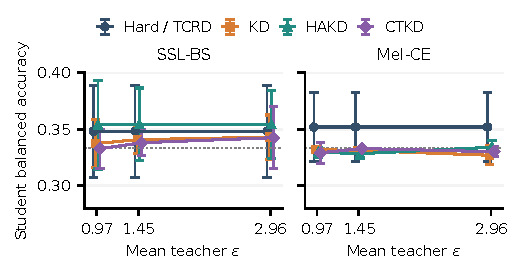
\includegraphics[width=\linewidth]{figure/FIG_stageD_hard_vs_kd_eps_2x2_groupedbars_seed_gradient_nogrid.pdf}
\caption{Small Common Voice privacy sweep (five-seed mean $\pm$ SD).}
\label{fig:cv_privacy_sweep_kd}
\end{figure}

\paragraph*{TCRD versus the simple teacher route}
\label{sec:cv_tcrd_routebalacc}
All health and teacher-dev BalAcc values lie below 0.45. TCRD/T-BAcc choose Hard throughout, and RC certifies Hard. This supplies no composite-score advantage: HAKD has higher SSL mean utility, while Hard leads for Mel. S-BAcc's SSL means are 0.3515/0.3513/0.3542 (Supplement III-C).

Figures~\ref{fig:cv_perclass_kd_diagnostic}--\ref{fig:cv_weak_teacher_tcrd} show the class, privacy, and weak-teacher diagnostics for the same paired seeds. Error bars are sample SDs; dotted lines mark chance. Horizontal offsets in the privacy plot separate methods sharing a budget. Concentrated predictions can accompany lost class-balanced utility.

\begin{figure}[t]
\centering
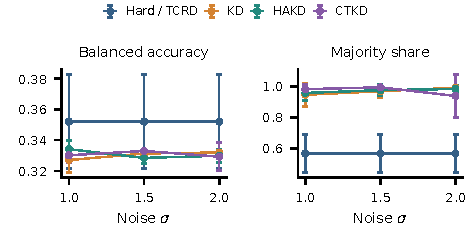
\includegraphics[width=\linewidth]{figure/cv_weak_teacher_tcrd.pdf}
\caption{Weak Mel-CE teachers: paired student utility and prediction concentration.}
\label{fig:cv_weak_teacher_tcrd}
\end{figure}

\begin{table}[t]
\centering\scriptsize\setlength{\tabcolsep}{1.4pt}
\caption{Small Common Voice routing diagnostics.}
\label{tab:app_cv_routing_diagnostics}
\begin{tabular}{llcccc}\toprule
Family & Policy & $\sigma=1$ & $\sigma=1.5$ & $\sigma=2$ & H/A/K\\
 & & \multicolumn{3}{c}{Macro-F1 / MajPred} &\\\midrule
\csname @@input\endcsname{restored_tables/routing_diagnostics.tex}
\bottomrule\end{tabular}
\end{table}
\begin{table}[t]
\centering\scriptsize\setlength{\tabcolsep}{3.3pt}
\caption{SSL-BS privacy sweep and paired KD gains.}
\label{tab:app_cv_privacy_sweep_gain}
\begin{tabular}{rrrrrrr}\toprule
$\sigma$ & $\bar\varepsilon$ & Hard & KD & $\Delta B$ & $\Delta F$ & $\Delta M$\\\midrule
\csname @@input\endcsname{restored_tables/privacy_gain.tex}
\bottomrule\end{tabular}
\end{table}

In Table~\ref{tab:app_cv_routing_diagnostics}, H/A/K count Hard/HAKD/KD decisions. Table~\ref{tab:app_cv_privacy_sweep_gain} gives mean $\varepsilon$, Hard/KD BalAcc, and KD-minus-Hard BalAcc/Macro-F1/MajPred differences in percentage points. Lower MajPred need not imply better classification.

\paragraph*{Additional Mel-BS condition}
Ten separately cached Mel-BS teachers at $\sigma=1,1.5$ give all-negative KD gains, means $-0.0265/-0.0262$; TCRD selects Hard. Supplement III-C specifies this distinct condition.

\subsection{VCTK: Paired Release and Alternative Supervision}
\label{sec:vctk_release}
Table~\ref{tab:vctk_release} includes directly released DP teachers and non-DP CE/BS controls matched on architecture, split, four epochs, optimizer and dev selection. TCRD selects Hard in all three seeds, avoiding negative mean KD gain but rejecting a small positive seed-wise gain. Near-chance utility makes this a limited-support stress test.


\begin{table}[t]
\centering
\caption{Cross-dataset release and VCTK controls (percent scores).}
\label{tab:vctk_release}
\label{tab:cross_dataset_summary}
\scriptsize\setlength{\tabcolsep}{2pt}
\begin{tabular}{llcccc}
\toprule
Dataset & Model & Acc & BalAcc & MF1 & MajPred\\
\midrule
VCTK & Non-DP CE & 22.5(5.1) & 22.5(5.1) & 14.0(2.0) & 70.3(27.3)\\
VCTK & Non-DP BS & 28.6(3.4) & 28.6(3.4) & 17.5(5.2) & 66.9(23.6)\\
\midrule
\csname @@input\endcsname{restored_tables/cross_dataset.tex}
\midrule
VCTK & CTKD, global & 20.6(8.2) & 20.6(8.2) & 13.5(5.7) & 61.9(10.2)\\
VCTK & S-BAcc & 25.3(4.3) & 25.3(4.3) & 16.6(4.9) & 78.3(16.6)\\
VCTK & PATE & 25.6(11.1) & 25.6(11.1) & 16.7(7.6) & 60.8(9.6)\\
VCTK & PATE + labels & 28.9(5.5) & 28.9(5.5) & 17.2(6.6) & 72.5(21.4)\\
\bottomrule
\end{tabular}
\end{table}

\begin{figure}[t]
\centering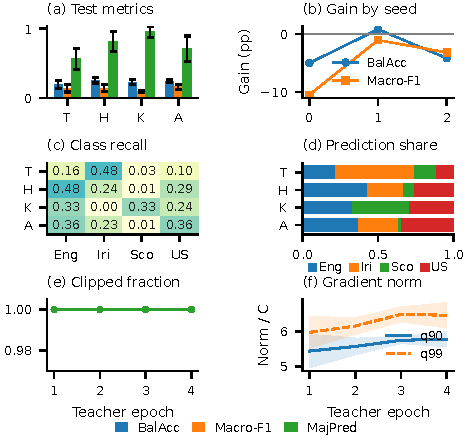
\includegraphics[width=\linewidth]{figure/vctk_main_rich_figure.pdf}
\caption{VCTK paired release and training diagnostics.}
\label{fig:app_vctk_main}
\end{figure}

In the diagnostic figures, T/H/K/A denote teacher/Hard/KD/HAKD. Figure~\ref{fig:app_vctk_main} averages English/Irish/Scottish/US class diagnostics over three seeds. Gains compare paired KD and Hard students; pre-clipping gradient quantiles show mean $\pm$ SD, normalized by $C$. Clipping fraction describes optimization, not routing utility. These public-benchmark gradient diagnostics are not DP release outputs.


Global-T CTKD uses the published temperature and gradient-reversal mechanism under matched training. The two explicit uncertainty/linear-temperature probes are not reproductions (Supplement II-B). PATE matches features, student architecture, initialization/order, five epochs and reported privacy bound. Adding permitted labels raises its mean above Hard/TCRD, with substantial three-seed variation; matching bounds does not equate privacy mechanisms (Supplement II-F).

\paragraph*{HAKD and health components}
Uniform/confidence/class HAKD obtains BalAcc $0.228/0.253/0.244$, versus instance HAKD's 0.239; full SDs and formulas appear in Supplement II-B. This sensitivity does not identify a uniquely optimal weight.

Ten component settings mostly select Hard. Dispersion alone selects HAKD once, lowering mean BalAcc to 0.242. Strict-pair health--gain Pearson/Spearman correlations are $(-0.965,-1.000)$, versus $(0.479,0.500)$ for BalAcc. Three seeds do not establish predictive increment (Supplement II-D).

\subsection{Uncertainty and Threshold Sensitivity}
\label{sec:uncertainty_results}
Development sizes $30/60/120$ cross four fixed threshold pairs. Retraining uses each restricted set throughout selection and calibration: nine teachers, 27 students. Defaults select Hard; near-boundary RC fallback can improve or reduce utility. Supplement II-C reports the full grid and earlier overlapping held-out-health checks, which do not establish population coverage.

\subsection{Other Transfer Conditions and Release Cost}
\label{sec:cross_dataset}
\paragraph*{Fixed-backbone weak teachers}
Five-seed VCTK Mel-CE health spans 0.1278--0.3123. Hard/KD/HAKD BalAcc is $0.2633/0.2733/0.2667$: weak hard predictions can still support useful KD (Supplement II-E).

\paragraph*{Heterogeneous teacher and student}
For frozen HuBERT-to-mel transfer, TCRD chooses Hard (BalAcc 0.2306), below KD (0.2750), CTKD (0.3111) and S-BAcc (0.2722). Supplement II-E reports all paired means/SDs and the replayed privacy budget.

\paragraph*{Emotion classification}
IEMOCAP~\cite{busso2008iemocap} uses open WavLM features.\footnote{\url{https://doi.org/10.5281/zenodo.17803295}, D. Yohanes and A. Chowanda, CC BY 4.0; raw USC audio has separate terms.} Removing unidentified rows and pooling identified variants yields 5,531 utterances, speaker-disjoint across private/aux/dev/test (3,259/1,031/590/651). Five-seed Hard/KD/HAKD BalAcc is $0.478/0.506/0.489$, teacher PRV $\varepsilon=1.840516$, $\delta=10^{-5}$. Both routes select Hard throughout, excluding useful KD (Supplement III-A--B).

\begin{figure}[t]
\centering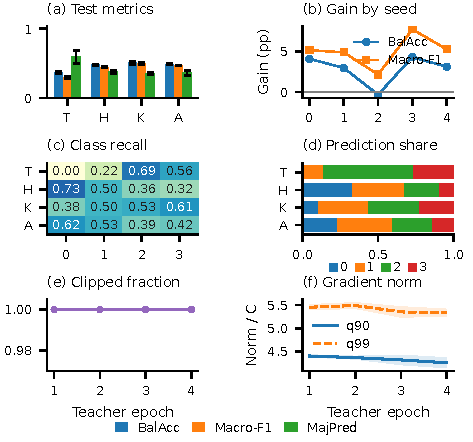
\includegraphics[width=\linewidth]{figure/ieo_iemocap_composite.pdf}
\caption{IEMOCAP paired release and training diagnostics.}
\label{fig:app_iemocap_main}
\end{figure}
\begin{figure}[t]
\centering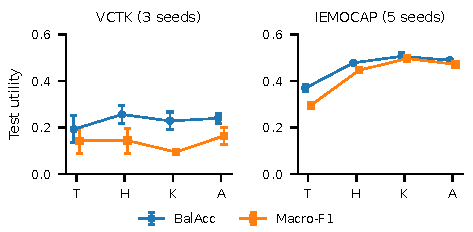
\includegraphics[width=\linewidth]{figure/vctk_iemocap_summary.pdf}
\caption{Cross-dataset teacher and student utility (mean $\pm$ SD).}
\label{fig:vctk_iemocap_summary}
\end{figure}

Figure~\ref{fig:app_iemocap_main} averages five seeds, retains released class IDs 0--3, and shows all four teacher epochs. Figure~\ref{fig:vctk_iemocap_summary} compares methods within each protocol; positive IEMOCAP KD gain contradicts exclusion based solely on low health.

\paragraph*{Release overhead}
The 108 matched warm-cache measurements comprise two small-archive model families, three seeds, three repeats and six policies, with 15 student epochs and CUDA synchronization. TCRD/S-BAcc take $0.218/0.790$~s (SSL), $0.738/2.319$~s (Mel); S-BAcc trains three candidates. Supplement II-F reports every policy, health overhead and memory. These all-Hard-route timings exclude common teacher/feature costs and do not describe CV17's 80 epochs.
